\documentclass[11pt]{article}
\usepackage{lmodern}
\usepackage{amssymb,amsmath}
\usepackage[framemethod=tikz]{mdframed}
\usepackage{ifxetex,ifluatex}
%\usepackage{fixltx2e} % provides \textsubscript
\usepackage{xr} % referencing external ducument
\ifnum 0\ifxetex 1\fi\ifluatex 1\fi=0 % if pdftex
  \usepackage[T1]{fontenc}
  \usepackage[utf8]{inputenc}
\else % if luatex or xelatex
  \ifxetex
    \usepackage{mathspec}
  \else
    \usepackage{fontspec}
  \fi
  \defaultfontfeatures{Ligatures=TeX,Scale=MatchLowercase}
\fi
% use upquote if available, for straight quotes in verbatim environments
\IfFileExists{upquote.sty}{\usepackage{upquote}}{}
% use microtype if available
\IfFileExists{microtype.sty}{%
\usepackage{microtype}
\UseMicrotypeSet[protrusion]{basicmath} % disable protrusion for tt fontshttps://de.overleaf.com/project/5e85b0680d0bed00011ea790
}{}
\usepackage[margin=1in]{geometry}
\usepackage{hyperref}
\hypersetup{unicode=true,
            pdftitle={Title: Human Neandertal Admixture dating limits MBE Supplements},
            pdfauthor={Leonardo Nicola Martin Iasi (Max Planck Institute for Evolutionary Anthropology, MPI EVA), Dr.~Benjamin Marco Peter (MPI EVA, benjamin\_peter@eva.mpg.de)},
            pdfborder={0 0 0},
            breaklinks=true}
\urlstyle{same}  % don't use monospace font for urls
 
%\usepackage{natbib}
%\bibliographystyle{References/my_abbrvnat}
%\setcitestyle{authoryear,open={(},close={)}}

\usepackage{graphicx,grffile}
\makeatletter
\def\maxwidth{\ifdim\Gin@nat@width>\linewidth\linewidth\else\Gin@nat@width\fi}
\def\maxheight{\ifdim\Gin@nat@height>\textheight\textheight\else\Gin@nat@height\fi}
\makeatother
% Scale images if necessary, so that they will not overflow the page
% margins by default, and it is still possible to overwrite the defaults
% using explicit options in \includegraphics[width, height, ...]{}

\setkeys{Gin}{width=\maxwidth,height=\maxheight,keepaspectratio}
\IfFileExists{parskip.sty}{%
\usepackage{parskip}
}{% else
\setlength{\parindent}{0pt}
\setlength{\parskip}{6pt plus 2pt minus 1pt}
}
\setlength{\emergencystretch}{3em}  % prevent overfull lines
\providecommand{\tightlist}{%
  \setlength{\itemsep}{0pt}\setlength{\parskip}{0pt}}
\setcounter{secnumdepth}{0}
% Redefines (sub)paragraphs to behave more like sections
\ifx\paragraph\undefined\else
\let\oldparagraph\paragraph
\renewcommand{\paragraph}[1]{\oldparagraph{#1}\mbox{}}
\fi
\ifx\subparagraph\undefined\else
\let\oldsubparagraph\subparagraph
\renewcommand{\subparagraph}[1]{\oldsubparagraph{#1}\mbox{}}
\fi

\usepackage{setspace}
\onehalfspacing
\usepackage[left]{lineno}
\linenumbers
\usepackage[none]{hyphenat}
\usepackage{amsfonts}
\usepackage{amssymb}
\usepackage{graphicx}
\usepackage{float}
\usepackage{xcolor}

\floatplacement{figure}{H}
\begin{document}

We thank the editor and all three reviewers for their very constructive feedback. While working on the revised manuscript, we substantially altered the derivation and presentation of the theoretical results. This was done with substantial contributions from \textbf{Harald Ringbauer}, whom we added as a co-author. As a result, we feel that the current version of the manuscript is much improved, has a much clearer presentation and  we hope we satisfactorily address all major issues raised during the review process.

In particular, we made the following major changes:
\begin{itemize}
    \item In response to the apparent disconnect between theory and application noted particularly by reviewer 1, we completely reworked the \textbf{theory section}. We now derive the connection between segment length distribution and ALD explicitly (\section{Appendix B}); showing that the two are direct functions from each other. To keep the presentation short, we added an \textbf{Appendix} where we present detailed computations.
    \item We also added a second \textbf{Appendix} where we detail the effect of the simplifications we made, and how the theory were to change if one incorporated e.g. genetic drift, particularly to address concerns raised by reviewer 3.
    \item We now focus more on model choice, as suggested by reviewer 1. For this purpose, we added a new \textbf{Figure 2}, with model-choice results under an idealized scenario. 
    \item We completely reworked \textbf{Figure 3}, to also include model choice between the simple and extended pulse model, and comparisons between segment-based inference and ALD inference (as suggested by reviewer 1), changed the parameter setting to one more directly relevant to Neandertal gene flow (as suggested by reviewer 2), and, in panel C adding curves showing the fit of the data to the predictions (as suggested by reviewer 3).
    \item We redid all simulations, in an attempt to improve the efficiency of segment-based inference. We also updated the fitting function (following a comment by reviewer 3).
    \item We changed the \textbf{Comparing Effect Size estimates} section based on feedback from reviewer 3. We added a downsampling scenario (just 5\% of SNPs), and added a second GLM investigating the accuracy of our ALD estimates (not just the bias). 
    \item We removed the old figure 2, which discussed the accuracy of estimated admixture times (using ALD) for simulations under both models. This information is now contained in the much more comprehensive Figure 3. 
\end{itemize}

We also made a large number of smaller changes based on the reviewer feedback. Please see our detailed responses below.

\section{Reviewer 1}\label{Reviewer 1}
Comments to the Author
Overall Summary 

The authors propose a statistical model to better characterize the dynamics of introgression, with an empirical focus to the challenge of better understanding the Neandertal introgression into modern humans. The extension allows for a more relaxed model, accounting for not only the mean time of introgression but the duration over which this introgression occurred. This extension moves beyond the commonly used assumption of a single “pulse” of admixture in the literature and retains an analytical tractability that has not previously been applied in the field. 

The authors focus a substantial amount of effort to characterize the ability to infer the mean admixture time as well as the admixture duration in their model, finding that the mean time to admixture can be reliably estimated in the simulations performed to mimic the scenario of Neanderthal admixture into humans. The authors highlight that the duration over which admixture occurred (their novel contribution) is less reliably inferred. Through their simulations the authors also quantify the impact of mis-specified recombination rate estimates and their contribution to estimation error of the mean admixture time. This technical impact of the recombination map has been shown previously, but the authors here describe it in tandem with numerous other technical covariates.  The authors also apply their method to admixture LD data from Neanderthals and modern European individuals from the 1000 Genomes project,  concluding that there is little power to distinguish between an admixture duration of 2500 generations and a pulse admixture event. 

Overall, I do believe that the authors have brought a useful and tractable model to bear on the problem of inferring the dynamics of admixture from multi-locus population genetic data. However, as much of the argumentation (and motivation) in the paper is focused on being able to distinguish between the “pulse” and “extended pulse” models, I believe that more formal model comparisons between these two scenarios is warranted (see Major comments below). A secondary concern is that in the manuscript the model is derived for admixture segments as well as admixture LD, but almost no attention is placed on the admixture segment -based estimation in the subsequent sections to compare the relative value of each of these data summaries.

While I believe the paper in its current form has intellectual merit and would be valuable to publish, it has a number of major shortcomings that are worth addressing prior to being accepted. Therefore, my recommendation would be that major revisions are required and the manuscript be resubmitted. Please see my detailed comments and considerations below: 

\paragraph{1.}
A key contribution that I would have hoped to get out of the manuscript is the power to reject the model of ``pulse admixture’’ given data simulated under a non-pulse model. To evaluate the power to detect a difference from $t_d$ = 1 (which is equivalent to the pulse model) in a likelihood-ratio test framework. This would assume a best-case scenario of no noise in the estimation of segment lengths, but would help inform the reader of the parameter regimes that are identifiable in the model. In my view this analysis is essential because it provides statistical evidence for how seriously I should take the claims made in the real data analysis.

\paragraph{2.}
A secondary question that is analytically tractable is how the power described above is shaped by the time-since admixture ($t_m$), which is implied by the statements that requiring samples closer to the time of admixture would be helpful for future inference (line 20 in the abstract for example). This would be useful to quantify what kind of data might be necessary to reject the model of pulse admixture (or if it is even possible at all with current human data parameters?). As this is a claim vaguely made in the paper – I believe that a statistical evaluation of the power to reject the pulse model with data from different time-points post-admixture. 

\paragraph{Answer to 1.1 and 1.2}
We agree that these are two important points that were poorly supported in the previous version of the manuscript. We performed an analysis addressing these two points, assuming fragments are fully observed (new \textbf{Figure 2}) as suggested in point 1, and sample at present-time and 50 generations after gene flow ended.

Our results show that from present-day data, even 100,000 admixture segments are not sufficient to distinguish admixture event spanning \~400 generations from a single pulse; whereas an event spanning 20 generations is detectable 50 generations later. This pattern is consistent for less data, and supports the previously intuitive argument that ancient DNA would help us better estimate the duration of gene flow.


\paragraph{3.}
Is there a difference in the power to reject the “pulse model” if one uses ALD at different length scales or realized segments? This would place clearer value on one summary statistic over the other for pursuing further inference in aDNA datasets. 

\paragraph{4.}
The focus in the paper is to distinguish between models of an extended duration of admixture using the decay of “admixture LD” but little attention is paid to the model using segments, although the authors detail this in the derivations first. The admixture LD is easier to calculate from data to avoid haplotype phasing, but in theory segments are detectable (Skov et al 2018). In the simulations detailed using msprime (Kellher et al 2016), it should be possible to directly use the introgressed segments for this task as well. In my view the authors should either entirely describe the results in terms of ALD, and making this more explicit in the section on Results/Simulations to say that this is the specific summary statistic that is presented throughout the results or to include supplementary results where the summary statistic of admixture segment lengths are used as well. 



\paragraph{Answer to 1.3 and 1.4}
We agree that these are valid points, and we changed the manuscript throughout to give a beetter balance between segments and ALD based results. 

In the \textbf{Theory section}, we now handle the segment length distribution and ALD equally, and we now derive both statistics (also based on feedback we got from Shai Carmi and Harald Ringbauer based on our preprint, that the previous derivation was slightly wrong).

In the analysis, we now added \textbf{Figure 3} in which we perform model comparisons and parameter estimates using both the ``true'' (simulated) segments, inferred segments (using the method from Skov et al. 2018) and ALD. We find that at the time-scale of interest (i.e 1,500 generations ago), fragment length identification is very sensitive to noise and leads to very poor performance for the inferred segments. This is why we focus on ALD for inference. 

We did not investigate ALD at multiple scales because for these admixture time scales the ALD-curve quickly reaches values extremely close to zero, so we would not think that this makes a substantial difference in the analysis. 



\subsection{Minor Comments}\label{Minor Comments}

Page 2 – line 52: avoid starting a sentence with “It” as it obscures the subject of the sentence, I think a more appropriate start would be “Uncertainty in the timing of gene flow also would affect …”

\textbf{Answer:} we changed it to "More certainty in the timing of gene flow also would affect  assumptions about introgressed allele frequencies and their distribution in present-day human genomes and conclusions drawn about the phenotypic effects and selective pressures of introduced alleles."

There is an error in notation on page 11- line 3: should be “tm” instead of “td” I believe.

\textbf{Answer:} The section where the error occurred is replaced by the new section "Population genetic model comparison"

A typo in the caption for Table S1: “standart” vs. “standard”

\textbf{Answer:} This table is updated and the error is corrected for both tables (Supplement Table 1 and 2) it reads "Standard Model"

A suggestion on the formatting for Table S2 would be to include the model estimates as the columns (and the different scenarios as rows), and the confidence intervals as part of the entries for the estimates in brackets / parentheses. The reader should be able to readily compare the same parameter across these fits by just looking at a single column. 

\textbf{Answer:} We restructured the table (now Supplement Table 3) as suggested.

There are several comments with regards to the structure and layout of the provided software code:


\paragraph{code}
Improve documentation for the `fit-extended-pulse` and `fit-simple-pulse` functions to better describe the inputs. I would recommend using the `roxygen` formatting for documentation to make the code more readable and useable. 
One suggestion would be to provide an example input for these functions within the repository to help the end user understand more clearly the required data table format. 
I would suggest a “requirements.md” or “requirements.txt” file in the main directory of the code to inform the user of the libraries required to import (and their versions if possible).

\textbf{Answer:} 

\section{Reviewer 2}\label{Reviewer 2}
Comments to the Author
In their manuscript, Iasi & Peter introduce an extended admixture pulse model that allows for joint estimation of the timing and duration of gene flow. Using simulations, the authors show how the estimates of timing and duration of gene flow are affected by different model assumptions and convincingly show that the estimates for the mean time of admixture are largely robust to details of the gene flow models. Authors then apply their method to Neandertal data and conclude that all tested scenarios (with different admixture durations) are compatible with observed data.

In addition to the careful examination of the extended admixture pulse model with simulations, one of the strongest aspects of this work is the discussion about the implications of their findings to the interpretation of previous dates for the Neandertal-Human introgression and for the understanding of selection on introgressed Neandertal haplotypes. I thoroughly enjoyed reading this manuscript and believe the implications of their work are relevant for the advance of our understanding of Neandertal introgression, in addition to representing a theoretical advance over previous admixture models. Below I list my concerns with this manuscript. 

\paragraph{1.}
My main concern relates to the “Application to Neandertal data.” My understanding of the manuscript title (An extended admixture pulse model reveals the limits to the dating of Human-Neandertal introgression) is that the extended model provides the limits (or bounds) for the dating of introgression. I do not think that this manuscript shows that. Instead, it seems like the application to Neandertal data shows that there is little power to differentiate tested scenarios (with varying gene flow durations). Perhaps the word “limits” in the title refers to the *limitations* of the model? I would like to hear from the authors about their intent and, if my understanding of the title is correct (i.e., limits == bounds), then I would like to see a more detailed discussion about this issue in the manuscript see comments below.

\paragraph{Answer to 2.1}
As non-native English speakers, we were not aware of the linguistic subtlety between ``limits'' and  ``limitations'', and suspect that many readers also will not be too concerned about this. To avoid ambiguity, we changed the title to ``An extended admixture pulse model reveals the limitations to Human-Neandertal introgression dating''. The latter change was necessary to remain under the 100-character title limit.

\paragraph{2.}
Overall, I think this subsection of Results is a bit underwhelming and somewhat disconnected from the part where authors examine their model with simulations. Given how the problem is introduced and the manuscript is presented, I would expect a more thorough examination of both the duration and mean time of Neandertal-human introgression. I think it is worth mentioning in the “Application to Neandertal data” section what are the estimates for the mean time of admixture and how they compare with published data. I understand this has been reported in previous studies, but I believe it would be important to report the estimates using their methods in a paper like this.

\paragraph{Answer to 2.2}
We do report all major previous (genetic) estimates of Neandertal gene flow dates in the introduction (section \textbf{Neandertal gene flow estimates}). We now also briefly discuss our results, and the inability to distinguish various events in the results section \textbf{Application to Neandertal data}.

We also added a section in the discussion where we explicitly compare our estimates with previous estimates, and discuss the implications:

\begin{mdframed}[hidealllines=true,backgroundcolor=grey!20]
Our estimate of the tm for Neandertal gene flow of 1,682 generations corresponds to a mean time estimate of 49ky (assuming a generation time of 29 years), with bounds of 44-54ky. This is in almost perfect agreement with the previous result of Moorjani 2016, which is based on largely the same method. However, here we show that models of extended gene flow with td up to a thousand generations provide very similar fits to the data; and that marginally better fits are achieved with very long gene flows. However, these models all would have Neandertals survive until around 30kya, whereas archaelogical evidence for Neandertals surviving beyond 40ky is increasingly sparse Hublin 2017, so that these models of extremely long gene flow might be rejected on these grounds.\end{mdframed}

\paragraph{3.}
I would also like to hear from the authors the reasons why the specific scenarios were chosen for the simulations. Since the paper focuses on Neandertal-Human introgression and the range for the dating of this event is well known (37-86kya, 41-54kya, or 50-60kya as reported by the authors), then I would expect the simulations to cover this range. Perhaps I missed something, but the simulated scenarios seem to include mostly very recent dates for introgression. The few examples where mean time of admixture match what is known for the Neandertal-Human introgression use the same duration of gene flow (800 generations). How does the inference work for shorter durations? It would be great to see with simulations if the estimates for the duration of admixture are robust for an admixture time that matches the expected range for Neanderthal introgression. Perhaps the application to the data does that already, but still, it is good to see how good the inferences for plausible scenarios are especially considering different admixture durations.

\paragraph{4.}
Generally speaking, I miss some discussion about the applicability of this model to the study of other events in human history/evolution and beyond humans.


\paragraph{Answer to 2.3 and 2.4}
We agree that the scenarios chosen for simulations in the previous version of the manuscript did not reflect a scenario of Neandertal admixture very well. We now changed this that we first study a scenario directly relevant to Neandertal gene flow $t_m=1,500$  with various gene flow durations (\textbf{Figures 2 and 3}). The previous Figure 4 (now \textbf{Figure 6}) was moved further back to emphasize that there we study parameter settings where parameter inference works much better, but, as pointed out, is not directly applicable to Neandertal admixture.

We also expanded  the discussion towards this, with the  first paragraph of the introduction now reading:

\begin{mdframed}[hidealllines=true,backgroundcolor=grey!20]
In this paper, we develop a new population genetic model for dating extended pulses of gene flow. One appealing feature of our model is that it has just two parameters, that can be interpreted as the mean time and duration of gene flow; which leads to simple closed form solutions, and we show that both an instantaneous pulse and continuous migration models can be thought of as special cases where the duration is extremely short or long, respectively. This makes this model generally applicable beyond gene flow between Neandertals and humans, which was the motivation and focus of this study. In fact, we find that we have much more power to investigate recent gene flow, so that this model should be particularly powerful if gene flow has been very recent. One restriction is that we assume that the overall amount of introduced material is low, and that we ignore the effects of genetic drift and selection.\end{mdframed}



\subsection{Minor Comments}\label{Minor Comments}

Minor comments:
Consider adding “on average” to the first sentence of the abstract (referring to the percentage of Neandertal DNA).

\textbf{Answer:} In our view, 2\% -3\% is a rough range, not an average.

Page 6, line 20. “Ti represents the time when segment Li entered the population” Would it be segment i instead of Li? 

\textbf{Answer:} Yes we changed it to: "We enumerate the admixture segments in a sample $i=1...n$. We denote the length of the $i$-th segment as $L_i$ and the time in the past when segment $i$ entered the population as $T_i$. We assume that the $L_i$ and $T_i$ are both realizations from more general distributions $L$ and $T$ that reflect the overall segment length and admixture time distributions, respectively."

Page 10, first line. Is it supposed to be tm=500 instead of td=500?

\textbf{Answer:} The section where the error occurred is replaced by the new section "Population genetic model comparison".


I do not follow what is described on page 13, first and second paragraphs. Would it be left panels instead of right? If that’s the case, then I can see that for panel C, not for panel A. If my reasoning is correct, then also change the reference to the right panels (not left) in the next paragraph.

\textbf{Answer:} The section where the error occurred is replaced by an updated version "Sampling closer to the admixture event". It reads now: "In panels A and B we increase both $t_m$ and $t_d$ at a similar rate, such that gene flow ends 50 generations before sampling ($t_{end}=50$, where $t_{end}= t_m - \frac{t_d}{2}$). In panels C and D $t_d$ is kept fixed at 800, but we increase $t_m$. We use the same four recombination scenarios as above, with one scenario of inference and simulation under constant recombination rate, and three scenarios with simulations using a variable recombination map, with inference using the same, a slightly different and non recombination map, respectively."

Page 12, line 56: I believe this is supposed to be Figure 4A. 

\textbf{Answer:} The section where the error occurred is replaced by an updated version "Sampling closer to the admixture event".

Typo? page 18, line 40/41 The effective… *and are* based on estimates…” 

\textbf{Answer:} This sentence is not in the manuscript anymore since we chenged the complex demographic model to the Skov et al. 2018 model.

Figure 2, panel A: Please use “Single pulse” instead of “Pulse.”

\textbf{Answer:} Figure 2 is replaced by Figure \ref{fig:figResult2}. The two admixture models are refert to as "simple pulse" and "extended pulse".


Figure 2, panel B: It seems like the color legend is redundant. Admixture duration is shown at the bottom of each column already, so no need to use the different colors. Also, it could be a bit distracting since you use the same colors for Figure 4. 

\textbf{Answer:} Figure 2 is replaced by Figure \ref{fig:figResult2}. The two color legend now are refering to the recombination map used for simulation and inference and which model is fitted to the curve.

Figure 3: why only the second dot is green?

\textbf{Answer:} 

Add units for time in figure 4. I suppose it is generations.

\textbf{Answer:} We included the sentence "All times are given in generations" in the legends of Figure \ref{fig:figResult2} and \ref{fig:Closer_sampling}.

References to supplementary figures lack the word “Figure.” 

\textbf{Answer:} We changed it and now throughout the paper it refers to as Supplement Figure or Supplement Table.

\section{Reviewer 3}\label{Reviewer 3}

Comments to the Author
Iasi and Peter developed a new method to estimate the duration of admixture using ancestral LD and segment length information. They investigated the accuracy of their method under different demographic models and applied it to human Neanderthal introgression. This is an interesting work touching a less studied direction, which I very much enjoy reading. The writing is clear and easy to follow. That said, I have multiple comments on the technical aspects of this work, which I wish to see addressed. 

\paragraph{1.}
As shown in their figures, the current version of this method is a biased method. Therefore, the single major concern I have about their paper is that it lacks explanations and investigations on the bias and variance of this newly proposed method. Hence some improvements are needed. In particular, why is it a biased method, and is it possible to improve on it further?

\paragraph{Answer to 3.1}
We agree that the biases in the estimates of $t_d$ and $t_m$ are unfortunate, and we note that the section \textbf{Comparing effect sizes for technical covariates} deals with investigating the various (technical) sources of bias of $t_m$. 

\paragraph{2.}
Simulation: the basic version of msPrime does not shine at simulating long-range LD in recent generations, and therefore it was recommended, when long-range correlations are used, the msPrime with Wright-Fisher extension should be used instead to overcome the biases in especially the recent time scale (see Nelson et al. 2020, PLoS genetics). When the admixture duration is long and extends to very recent time as in some of the simulations for the extended pulse model, and long-range information (LD, segment length) is used in inference, it might be essential to incorporate the WF extension in the simulation.Some of the biases perhaps would disappear with better simulation. It is also possible that a more realistic simulation would lead to even larger bias, which would also be essential to know.

\paragraph{Answer to 3.2}
We verified that we are outside the parameter range where this is a concern by redoing the most extreme scenario we use using either simulation scheme. We do not find any difference between the two models (see attached figure), so we feel confident that this is a very unlikely source of bias.

\begin{figure}
\centering
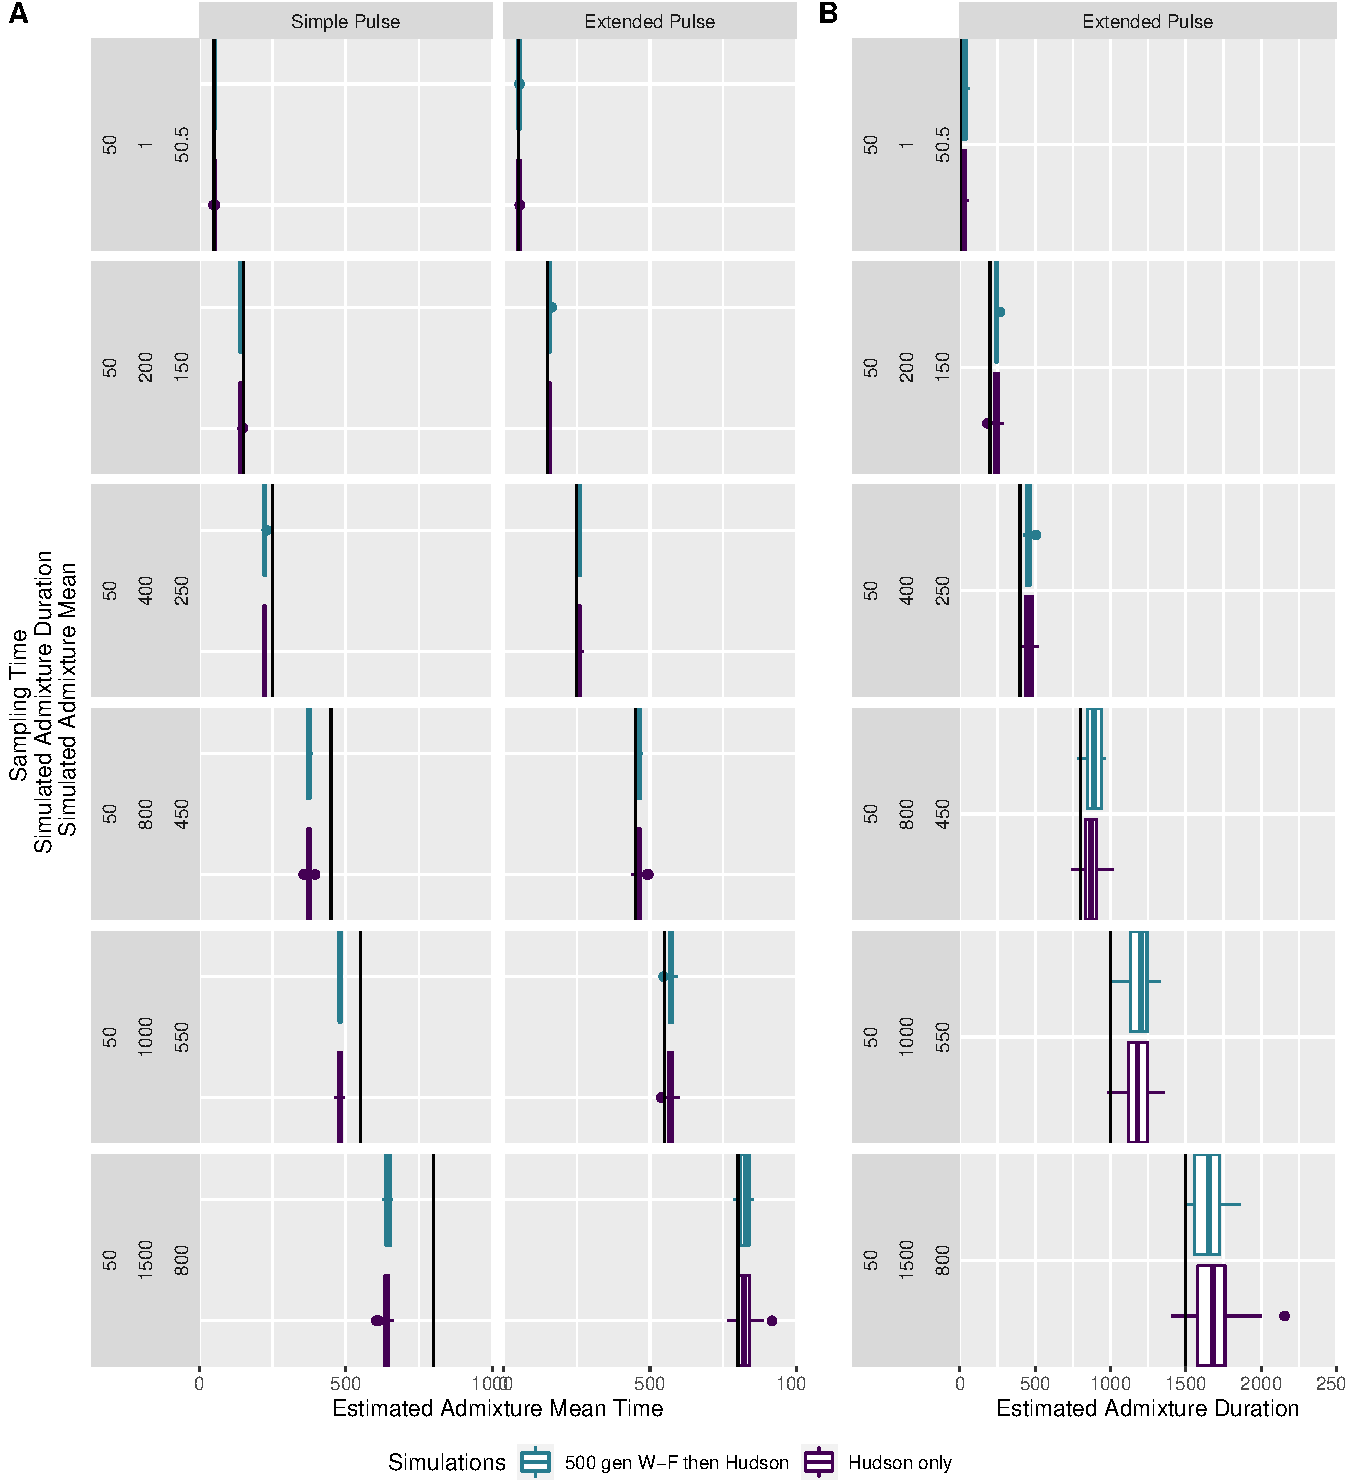
\includegraphics[width=16cm,height=18cm,keepaspectratio]{ATE_Revisions_files/figure-latex/figResult_WF_H_comp-1.pdf}
\caption{\label{fig:fig_R} }
\end{figure}

\paragraph{3.}
Model: I wonder if the authors decided to dismiss the admixture fraction too soon without giving enough justifications (on page 8 line 24-24). While this assumption that recombination within archaic segments can be ignored is perhaps justifiable in some previous work, this paper works on a more delicate problem, and subtle signals and biases matter more. To differentiate single pulse and extended pulse, fixed admixture fraction in a single pulse and increasing admixture fraction over time in the extended pulse is a signature of these different admixture models. I wonder if some of the biases in their method is related to this simplification. To elaborate, let’s assume total admixture fraction is $\alpha$, and recombination rate r, mean time of admixture T, under a single pulse model, the effective recombination rate which will affect the introgressed segment length with rate $(1-\alpha)$ rT, rather than rT. Because the authors convert the length to cM, the $(1-\alpha)$ factor would affect T and can lead to a directional bias as observed in single pulse model. Under the extended pulse framework, the recombination rate for segments entering human population at time t is:


$$R(t) = \int_{0}^{t}{\left(1-\alpha\ Pr(T=s)\right)r\ ds}$$,
 where 

$$Pr\left(T=s\right)=\ \int_{s}^{\infty}P\left(T=t\right)dt,$$

,where this P(T=t) is the same as the Eq. 7 in the paper.
 
$$  P(T_i=t)=\frac{1}{\Gamma(k)(\frac{t_m}{k})^k}t^{k-1}e^{-t\frac{k}{t_m}}$$
 
This should result in a simple transformation w.r.t $\alpha$. The point is that it seems the math would still be straightforward even when admixture fraction is included (or numerical integration could be used), then why not give it a try and see if the method could be improved further?

\paragraph{Answer to 3.3}
We do agree that these elaborations are intuitively reasonable, but to show where/if they hold we would have to develop an SMC or SMC'-like model in quite some detail, which we feel is beyond the scope of the current paper. Moreover, we found that with the way that we consider linkage disequilibrium separately, we are able to include the migration fraction in a much more direct way in our model. 

We hope that the clarifications made in the theory section (also motivated by other comments, see above), now make it more clear what the assumptions of our very simple model are.

In addition, we added an \textbf{Appendix} where we add many further details and outline some calculations if one chose to include the effects of genetic drift and recombination between introgressed material. In particular, we show that the ALD model we use can be motivated by the solution to a differential equation where ALD is introduced by gene flow, and decays by recombination. We also outline that replacement of previously introgressed material by new introgressed material could be accommodated in a framework very similar to the one suggested by the reviewer, but we do not pursue that further because we think the effect will be small.

Finally, we outline the standard theory (from Liang \& Nielsen 2014) for the single pulse and how recombination and drift would affect our inference, and show that the bias due to these factors is very moderate for our parameters of interest, in the order of 10\%.

Taken together, we hope that these clarifications as well as the appendix show that the bias introduced by our modelling assumptions are likely small.

\paragraph{4.}
Inference: It seems the parameter inference is made by non-linear least-square optimization when alternatively, some maximum likelihood optimizations could be used. Could the authors provide more information about how good the fitting is per simulation? In particular, if the simulated parameters may actually give a higher likelihood.

\paragraph{Answer to 3.4}
We are not aware of any likelihood-based inference framework based on ALD, as the resulting summary statistic is an (approximated) LD-decay curve. We note that all state-of-the-art methods for this purpose use least-squares techniques similar to what we are using here (ALDER; Loh et al. 2013, DATES Narasimhan et al 2018, Globetrotter, Hellenthal et al. 2014). If admixture segments were perfectly known, then likelihood-based inference can be performed, but the issue is in identifying the fragments, and to propagate the uncertainty in fragment estimation.

In \textbf{Figure 3C}, we now show the fitted curves for both true segments, inferred segments as well as the raw ALD data, to show that the fits are reasonable. We did also change the algorithm used in \texttt{nls} for \textbf{Figure 3 and 6} to include upper and lower boundaries. As the extended pulse model converges to the single pulse model when $k \to \infty$, there are some numerical issues to be considered. 

\paragraph{5.} 
Data: As primarily a new method paper, it would be nice to provide guidance about how much data is needed to make these inferences. 
How does the accuracy of ALD from ALDER affect the variance and bias in the inference? 
How does ascertainment of introgressed mutations affect the accuracy? 

\paragraph{Answer to 3.5}
We address these concern in \textbf{Figure 4} and section \textbf{Compariong effect sizes for covariates} by i) adding a ``downsampling''-parameter where we remove 95\% of SNPs, and ii) by fitting a second model where we compare the contributions of our modeling parameters on the mean absolute deviation. Somewhat surprisingly, we find that we get only slightly worse estimates from downsampled data, and that issues due to misspecification are much more important. 


\paragraph{6.} 
Discussion: I wonder if the first paragraph of the discussion could be rephrased a little bit. It seems obvious that the previous estimates are the CI rather than the bounds of the duration of gene flow. Is there any paper stating or interpreting them as the bounds of the duration of gene flow? It is also good to acknowledge and discuss that a method based on ALD or length of the segment might not be the ultimate method for addressing the admixture duration. An extended admixture affects coalescence time, site frequency spectrum, etc. Various aspects could be explored in the future.

\paragraph{Answer to 3.6}
We do agree that this should be phrased carefully, as it is a rather subtle point. What we were trying to say here is that if the single pulse model were correct, then the bounds on the estimates of $t_m$ are, in fact,  the bounds of when gene flow happened. So this is not a statistical error, but rather a case where the model is interpreted to literally. 

We found numerous papers that based their interpretations (partially) on this, in our eyes, flawed interpretation (see below).

Douka et al. 2019 "Denisovans at the site appear to have survived later than Neanderthals. Our modelled date estimate for the most recent Denisovan fossil (Denisova 3, 51,600–76,200 years ago) is earlier than published estimates of the date of Denisovan admixture into modern humans (44,000–54,00015 and 31,000–50,000 years ago16). If these admixture estimates are robust, then the Altai Denisovans may not have been the latest-surviving population."

Jacobs et al. 2019: "While the median block lengths of D1 and D2 are similar in Papuans (238 and 236 kb), their distributions are significantly different (Kolmogorov-Smirnov statistic = 0.15, p = $2.2 \times 10−6$). Exponential fitting of D1 and D2 haplotype lengths yields introgression dates of 29.8 kya (95 \% CI 14.4–50.4) and 45.7 kya (95 \% CI 31.9–60.7), respectively, which are younger, though overlapping with, previously suggested estimates for Denisovan introgression  (Malaspinas et al., 2016). The maximum likelihood introgression date for D2 introgression is 50 \% more ancient than the date for D1. Based on simulations, and given the greater statistical challenge of identifying shorter introgression blocks, we consider these dates to be probable lower bounds on introgression times, but with true dates no more than 15 \% more ancient.

D1 and D2 introgression times that overlap the timescale of modern human arrival and their variable dispersal across Papua raise the possibility that Denisovan introgression occurred after local populations of modern humans had differentiated."

Lazaridis et al. 2016: "The finding of little if any Neanderthal ancestry in Basal Eurasians could be explained if the Neanderthal admixture into modern humans 50,000-60,000 years ago11 largely occurred after the splitting of the Basal Eurasians from other non-Africans."

To make this point more clear, we rephrased this section as follows:

\begin{mdframed}[hidealllines=true,backgroundcolor=grey!20]
Previous estimates to date Neandertal-human gene flow have focused almost entirely on the mean time of gene flow using a simple pulse model, for which reasonably tight credible intervals can be estimated (Sankararaman et al, Moorjani et al). Under this model, the credible intervals of this time are bounds of when gene flow between Neandertals and early modern humans could have happened. 

Our estimate of the tm for Neandertal gene flow of 1,682 generations corresponds to a mean time estimate of 49ky (assuming a generation time of 29 years), with bounds of 44-54ky. This is in almost perfect agreement with the previous result of Moorjani et al 2016, which is based on largely the same method. However, here we show that models of extended gene flow with td up to a thousand generations provide very similar fits to the data; and that marginally better fits are achieved with very long gene flows. However, these models all would have Neandertals survive until around 30kya, whereas archaelogical evidence for Neandertals surviving beyond 40ky is increasingly sparse (Hublin 2017), so that these models of extremely long gene flow might be rejected on these grounds. 
\end{mdframed}
\end{document}